\documentclass{report}
\usepackage[T1]{fontenc}
\usepackage[margin=1.5 in]{geometry}
\usepackage[french]{babel}
\usepackage{graphicx}
\usepackage{hyperref}
\usepackage{fancyhdr}
\newcommand{\horrule}[1]{\rule{\linewidth}{#1}}
 \geometry{
 a4paper,
 left=30mm,
 right=30mm,
 top=30mm,
 bottom=28mm,
 }

\title{
		\vspace{-2.5in} 	
		\normalfont \normalsize \textsc{Haute École du paysage, d'ingénierie et d'architecture de Genève} \\ [25pt]
		\vspace{0.3in} 
		\horrule{2pt} \\[0.5cm]
		\LARGE \textbf{TP PROGRAMMATION TEMPS RÉEL:\\ BULLES}
		\vspace{1in}
		\horrule{2pt}
		
\includegraphics[scale=0.4]{images/bulles.jpg}
		\vspace{1in} 
}
\date{\today}
\author{
  \Large{Luc LAMBERT}\\
  \texttt{\small \href {mailto:luc.lambert@etu.hesge.ch}{luc.lambert@etu.hesge.ch}}
}
\begin{document}
\pagestyle{fancy}

\fancyhead[R]{TP PROGRAMMATION TEMPS RÉEL - BULLES}
\fancyhead[L]{Lambert Luc}
\cfoot{\thepage}
\maketitle %
%
\section*{Intérêts d'un RTOS}
L'intérêt d'utiliser un RTOS se résume à la gestion des timings ainsi qu'à la pseudo parralélisation des tâches.Toutes les tâches, de calcul de position et d'affichage des différents éléments, doivent être suffisament précisent pour que notre jeu ne soit pas saccadé. Le type coopératif est plus intéressant dans ce cas car toutes les tâches doivent s'éxecuter avant un temps donner. Il est donc plus simple, lors de la fin d'une itération de tâche que celle-ci passe la main à une autre tâche, sachant qu'il n'y a pas d'ordre dans l'éxécution des tâches.

\section*{État du projet}
Le programme est fonctionel, l'affichage des sprites, leurs déplacement, la gestion du score, le début et la fin de partie sont opérationels.

\section*{Anomalies du projet}
Plusieurs anomalies apparaisent une fois le projet lancé. Parfois la carte esclave se fige et on est obligé de reset la carte et de reflasher le programme esclave dessus. Autrement, après qu'une partie est été jouée lorsque des bulles explosent celle-ci font leurs animations plusieurs fois avant de disparaître. J'ai pensé que ce problème pourrait venir d'un sémaphore qui ne serai pas débloqué au bon moment. 

\section*{Traces et timings des tâches}
La charge maximale du CPU(U) est égale à : \\
\begin{tabular}{|l|c|r|}
    \hline
    Tâche & T & C \tabularnewline
    \hline
    $racket_m$ & 10 & 1870\tabularnewline
    \hline
    $racket_s$ & 10 & 1870\tabularnewline
    \hline
    $bubble_1$ & 30 & 5440\tabularnewline
    \hline
    $bubble_2$ & 30 & 5450\tabularnewline
    \hline
    $bubble_3$ & 30 & 5490\tabularnewline
    \hline
    $bubble_4$ & 30 & 5450\tabularnewline
    \hline
    $bubble_5$ & 30 & 5420\tabularnewline
    \hline
    $bubble_6$ & 30 & 5460\tabularnewline
    \hline
 \end{tabular}
$$ U = \sum{\frac{C_i}{T_i}}\leq1$$

On voit que la somme va être largement supérieur à 1. Je ne sais pas pourquoi les mesures des traces ci-dessous affiche des temps énormes. Alors que le jeu est fluide.

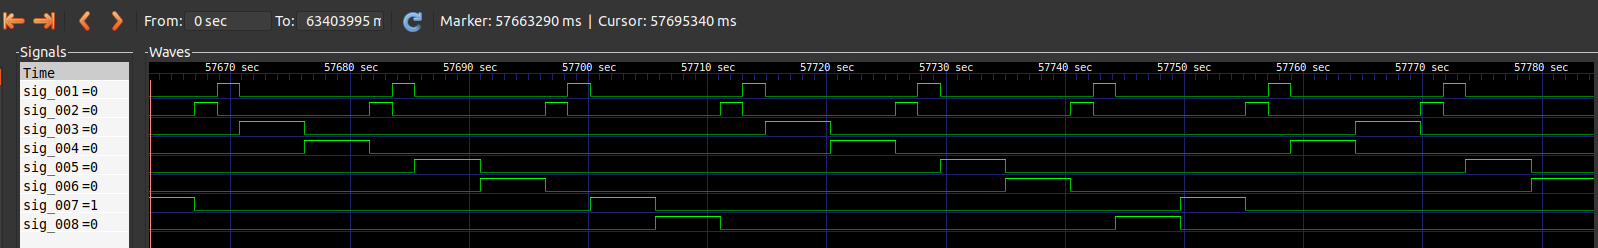
\includegraphics[scale=0.25]{images/traces.png}\\
L'image ci-dessus représente les traces laissées par chaque tâches de mon projet. Les 2 premières représentent les tâches liées à la gestion de la racket. Les autres correspondent aux bulles. On observe qu'il n'y a pas de dérive temporelle car toutes les tâches s'enchainent de manières régulières. Il y a tout le temps, trois fois les tâches de racket pour que toutes les tâches de bulles soient éffectuées. On sait qu'une tâche de racket doit s'éxecuter toutes les 10ms, tandis qu'une tâche de bulle, toutes les 30ms. On a bien un rapport de 3.


\end{document}


